\documentclass[a4paper,10pt,twocolumn,uplatex]{jsarticle}
\usepackage{style/nislab}

%---------------------------------------------------------------------
% レジュメ種別・日付設定(要変更)
% \type{} 1:修士論文諮問会 2:卒業論文発表会 else:月例発表会
\type{3}
\year{2021}
\month{7}
\date{10}

%---------------------------------------------------------------------
% ページ番号設定(要変更)
\setcounter{page}{9}

%---------------------------------------------------------------------
\begin{document}
%---------------------------------------------------------------------
% タイトル作成部分(要変更)
% \maketitle{タイトル}{title}{名前}{name}
\maketitle{ホームネットワークにおけるOpenFlowを用いた\\トラフィック監視によるセキュリティ向上}
{Improving Security by Monitoring Traffic Using OpenFlow in Home Networks}
{塚﨑 拓真}
{Takuma Tsukasaki}

%---------------------------------------------------------------------
\section{はじめに}
近年,IoT(Internet of Things)が注目を集めるようになり,今後あらゆるものがネットワークに接続され,利用されることが予想される.
それに伴い,ネットワーク内には様々な端末や機器が混在することになる.ホームネットワークは情報家電などの普及も加わり,その形態が多様化していくと考えられる.\par
しかし,IoTの登場で利便性が高まる一方で,これまでのネットワークに接続されていないモノが接続されることにより,セキュリティ上のリスクが高まっている\cite{guideline}.
IoTはセキュリティを考慮せずに開発されたものが多く,悪意のある攻撃者によるサイバー攻撃の標的になりやすく,特に不正アクセスが多発している.
これらが各種端末やネットワークごとに顕在した場合,個別に対処するとコストや時間がかかってしまうため,脅威に対し一括に対処する必要がある.
ホームネットワーク内には異なる規格のハードウェアやそれらに搭載される様々なアプリケーションが混在しているため,それら全てに対応したシステムの構築や更新を続けるのは困難である.
そのため,ホームネットワーク内で通信するのであれば,どの端末も必ず利用するネットワークを利用したシステムを構築することが望ましい.

%---------------------------------------------------------------------
\section{関連研究}
村上らは,OpenFlowを用いてホームネットワーク内に,動的な認証システムを構築し,不正アクセスによる被害を軽減する手法を提案した\cite{related}.
認証時に頻繁に利用される情報を用いることで,ネットワークに接続する端末を制限すると共に,万が一認証が突破された場合でも不正アクセスが検出できるシステムを構築した.
しかし,1度攻撃者に認証を突破された場合,不正アクセスを検出するまでに時間がかかると考えられ,ホームネットワーク内に不正アクセスが拡大してしまう問題点がある.
現在のスマートホームデバイスは,クラウド上のシステムと連携することで,デバイス間の連携を可能にしているが,今後はホームネットワーク内で閉じたデバイス間の通信によって連携を行う形になることが想定される\cite{d2d}.
デバイス間で直接通信を行う場合,各デバイスでどういったデバイスとの通信を受け入れるかアクセス制御を行う必要がある.
しかし,全てのデバイスがアクセス制御に対応しているとは限らず,デバイスの計算能力の制限によって実現できるアクセス制御に制限があったり,デバイスのソフトウェア自体の脆弱性によってアクセス制御が機能しない場合が考えられる.
同じホームネットワークに他の多くの機器が何の制限もなく接続されているという事実を利用して,個人情報の漏洩やサービスの操作など,悪意ある活動を行う可能性がある\cite{disap}.

%---------------------------------------------------------------------
\begin{figure}[!tb]
  \centering
  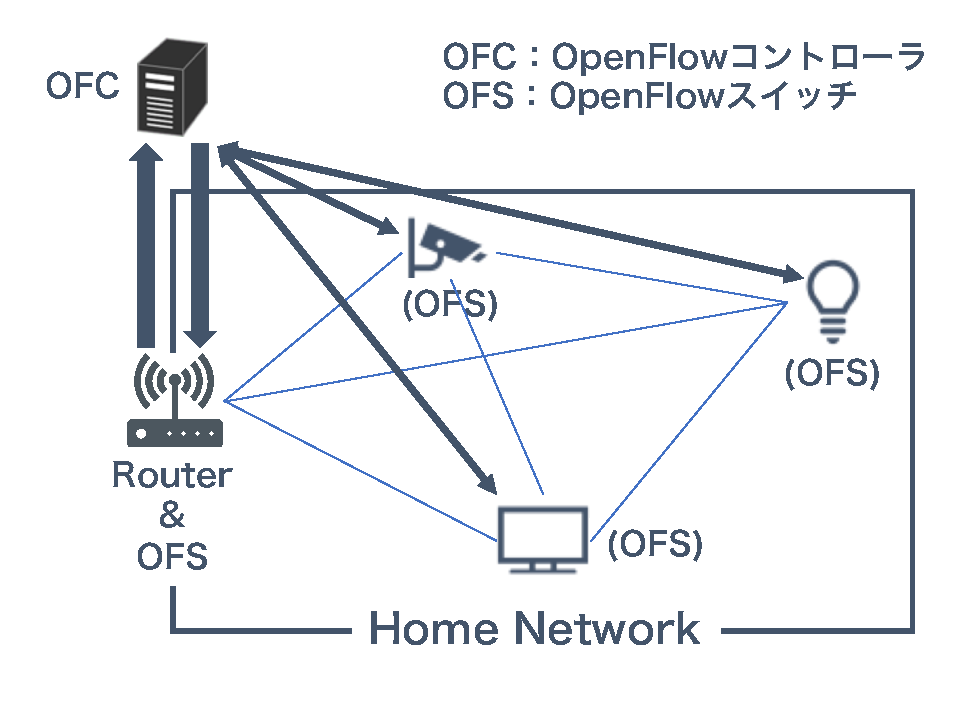
\includegraphics[width=\linewidth]{img/architecture.eps}
  \caption{提案手法のアーキテクチャ}
  \label{fig:architecture}
\end{figure}

%---------------------------------------------------------------------
\section{提案手法}
前述の問題点を受けて,不正アクセス拡大を防ぐことを考慮し,ホームネットワーク内においての検知も必要である.
本提案手法では,OpenFlowを利用することで,既存IoT機器や異なる規格などに対応でき,ホームネットワークに適した形で不正な通信の検知を実現する.
また,動的に接続を管理することで,不正通信による被害を軽減する.

\subsection{想定環境}
本提案手法のアーキテクチャを図\ref{fig:architecture}に示す.
ホームネットワークにおける閉じたデバイス間の通信,ルーター・デバイス間の通信を想定する.
また,デバイス数は一般的に利用されているルーターの推奨接続台数である10\textasciitilde15台を想定する.

\subsection{概要}
OpenFlowを用いて,トラフィック監視を行うことで,ホームネットワーク内で行われる通信を制限する.
既存IoT機器にOpenFlowスイッチの機能を導入することは困難であると考え,OpenFlowスイッチの機能を持った仮想デバイスを既存IoT機器の前に用意する.
通信が行われる際に,仮想デバイスを通して,OpenFlowコントローラに接続し,トラフィック情報から通信の許可を判断する.

\subsection{動作手順}
本提案手法の動作手順のシーケンス図を図\ref{fig:sequence}に示し,詳細を以下に述べる.

\begin{enumerate}
  \item 仮想デバイス(OFS)とOpenFlowコントローラは双方に対して,Echo Request/Replyメッセージを定期的に送信
  \item 接続要求機器は仮想デバイス(OFS)に通信
  \item 仮想デバイス(OFS)はOpenFlowコントローラに対して,Packet Inメッセージを送信
  \item OpenFlowコントローラはトラフィック情報を調査
  \item 正当な通信の場合,OpenFlowコントローラは仮想デバイス(OFS)に対して,許可メッセージとして,Flow Modメッセージを送信 \par 不正な通信の場合,OpenFlowコントローラは仮想デバイス(OFS)に対して,不許可メッセージとして,Flow Modメッセージを送信
  \item OpenFlowコントローラは送信元機器に対して,Packet Outメッセージを送信
\end{enumerate}

\subsection{トラフィック情報}
本提案手法で通信の許可を判断するトラフィック情報として,以下の3点を用いる.

\begin{itemize}
  \item パケットヘッダー
  \item パケットの長さ
  \item 周期性
\end{itemize}

%---------------------------------------------------------------------
\begin{figure}[!tb]
  \centering
  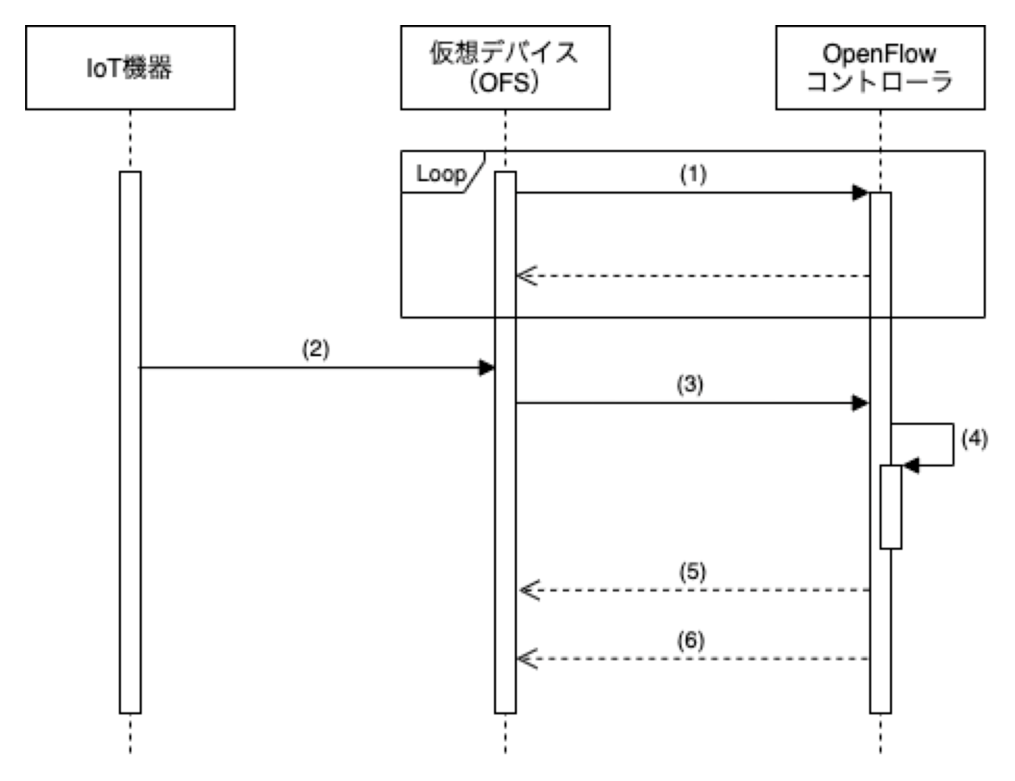
\includegraphics[width=\linewidth]{img/sequence.eps}
  \caption{動作手順のシーケンス図}
  \label{fig:sequence}
\end{figure}

%---------------------------------------------------------------------
\section{評価}

\subsection{評価項目}
本研究では,セキュリティと負荷を評価する.そのため,セキュリティ面では,正当なアクセスは通信が許可されるか,不正なアクセスは通信が許可されないかを実証する.
また,負荷面では,ネットワークに与える影響を測定したいため,スループットを評価する.

\subsection{評価シナリオ}
評価シナリオとしては,IoT機器が1対1,1対N,N対N($2\leqq N \leqq 15$)で通信を行っている状況を想定し,各状況において評価を行う.

%---------------------------------------------------------------------
\section{まとめ・今後の課題}
本稿では,ホームネットワークの形態の多様化からセキュリティ上の課題として,近年,増加傾向が見られる不正アクセスに着目した.
また,今後のスマートホームデバイスは,ホームネットワーク内で閉じたデバイス間の通信によって連携を行う形になることが想定される.
そこで本研究ではその対策として,OpenFlowを用いてホームネットワーク内で動的なトラフィック監視を行い,デバイス間通信における不正アクセスによる被害を軽減する手法を提案した.
本提案手法では,デバイスの前にOpenFlowスイッチの機能を持った仮想デバイスを配置し,トラフィック情報をOpenFlowコントローラで管理することで,不正アクセスを防ぐ.
\par
今後の課題としては,トラフィック情報の監視において,何を正当とし,何を不正とするのかの閾値と,具体的な検知手法を検討する必要がある.
また,本提案手法の評価において,セキュリティ面の評価が重要であると考える.
評価として,正当アクセスと不正アクセスをどれほど正確に判別できるか定性的な評価を行い,セキュリティの観点からの本提案方式の有用性を示したい.

%---------------------------------------------------------------------
% Bibliography
\footnotesize{
  \begin{thebibliography}{99}
    \bibitem{guideline} IoT推進コンソーシアム, 総務省, 経済産業省, "IoTセキュリティガイドライン ver 1.0", 2016.
    \bibitem{related} 村上萌, 中村嘉隆, 高橋修, "OpenFlowを用いたホームネットワークへの接続端末制御による不正アクセス防御手法の提案", 研究報告コンピュータセキュリティ(CSEC), Vol.2016-CSEC-72, No.29, pp.1-6, 2016.
    \bibitem{d2d} C. Vallati, A. Virdis, E. Mingozzi and G. Stea, "Mobile-Edge Computing Come Home Connecting things in future smart homes using LTE device-to-device communications", IEEE Consumer Electronics Magazine, Vol.5, No.4, pp.77-83, 2016.
    \bibitem{disap} M. Serror, M. Henze, S. Hack, M. Schuba, and K. Wehrle, "Towards In-Network Security for Smart Homes", Proceedings of the 13th International Conference on Availability, Reliability and Security (ARES 2018), No.18, pp.1-8, 2018.
  \end{thebibliography}
}

%---------------------------------------------------------------------
\end{document}
%---------------------------------------------------------------------
